\section{The Bipartisan Paxos Protocols}\seclabel{BipartisanPaxos}
The BPaxos protocols implement state machine replication. Informally, a set of
clients propose commands to a set of replicas, and the replicas execute the
commands in the same order (modulo reordering of non-conflicting commands). In
this section, we formalize state machine replication by way of generalized
consensus on conflict graphs. We then overview the common structure that
underlies all of the BPaxos protocols.

\subsection{Problem Description}
{\begin{figure}[h]
  \centering
  \tikzstyle{vertex}=[]
  \tikzstyle{arrow}=[thick, -latex]
  \tikzstyle{hidden}=[gray!50]

  \begin{subfigure}[b]{1.4in}
    \centering
    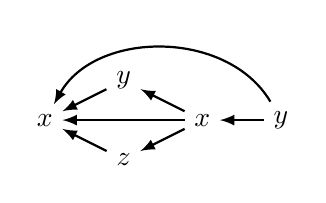
\begin{tikzpicture}
      \node[vertex] (x1) at (0, 0) {$x$};
      \node[vertex] (y1) at (1, 0.5) {$y$};
      \node[vertex] (y2) at (1, -0.5) {$z$};
      \node[vertex] (x2) at (2, 0) {$x$};
      \node[vertex] (z) at (3, 0) {$y$};

      \draw[arrow] (y1) to (x1);
      \draw[arrow] (y2) to (x1);
      \draw[arrow] (x2) to (y1);
      \draw[arrow] (x2) to (y2);
      \draw[arrow] (x2) to (x1);
      \draw[arrow, bend right=60] (z) to (x1);
      \draw[arrow] (z) to (x2);
    \end{tikzpicture}
    \caption{A conflict graph $C$}\figlabel{ExampleConflictGraph}
  \end{subfigure}%
  \hspace{1in}
  %
  \begin{subfigure}[b]{1.4in}
    \centering
    \begin{tikzpicture}
      \node[vertex] (x1) at (0, 0) {$x$};
      \node[vertex] (y1) at (1, 0.5) {$y$};
      \node[vertex] (y2) at (1, -0.5) {$z$};
      \node[vertex] (x2) at (2, 0) {$x$};
      \node[vertex, hidden] (z) at (3, 0) {$y$};

      \draw[arrow] (y1) to (x1);
      \draw[arrow] (y2) to (x1);
      \draw[arrow] (x2) to (y1);
      \draw[arrow] (x2) to (y2);
      \draw[arrow] (x2) to (x1);
      \draw[arrow, bend right=60, hidden] (z) to (x1);
      \draw[arrow, hidden] (z) to (x2);
    \end{tikzpicture}
    \caption{A suffix of $C$}\figlabel{ExampleSuffix}
  \end{subfigure}

  \caption{}
\end{figure}
}

Consider a set $\Cmd$ of commands and a binary reflexive relation $\conflict$
over $\Cmd$. We say two commands $x$ and $y$ \defword{conflict} if $(x, y) \in
\conflict$, and we say they are \defword{independent} otherwise. A
\defword{conflict graph} (over $\conflict$) is a directed acyclic graph such
that every vertex is labelled with a command and such that there exists an edge
between two vertices if and only if they are labelled with commands that
conflict (with respect to $\conflict$)~\cite{mazurkiewicz1995introduction}.

We associate every conflict graph with the set of command strings that can be
obtained by a reverse topological sort of the conflict graph. For example,
consider the conflict graph over $\conflict$ shown in
\figref{ExampleConflictGraph} where
  $\conflict = \set{(x, x), (x, y), (y, x), (x, z), (z, x)}$.
The conflict graph can be reverse topological sorted in two ways, yielding the
two command strings $xyzxy$ and $xzyxy$. Moreover, notice that these two
command strings can be obtained from one another by interchanging their second
and third commands. This is true in general. Any two command strings of a
conflict graph can be obtained from the other by repeatedly interchanging
adjacent independent commands. These sets of command strings are known as
Mazurkiewicz traces~\cite{mazurkiewicz1985semantics,
mazurkiewicz1995introduction} and formalize the orders in which replicated
state machines can execute commands while remaining in sync.

Let $G = (V, E, \varphi)$ be a conflict graph where $V$ is the set of vertices,
$E \subseteq V \times V$ is the set of edges, and $\varphi: V \to \Cmd$ is the
labelling function that assigns a command to every vertex. We say $G' = (V',
E', \varphi|_{V'})$ is a \defword{suffix} of $G$ if $G'$ is a subgraph of $G$
such that for every edge $(v_1, v_2) \in E$, if $v_1 \in V'$, then $(v_1, v_2)
\in E'$.

Generalized consensus on conflict graphs---first introduced
in~\cite{lamport1998part}---involves a set of processes known as
\defword{learners} attempting to reach consensus on a growing dependency graph.
More formally, given a set $\Cmd$ of commands and conflict relation
$\conflict$, we consider a set $l_1, l_2, \ldots, l_n$ of learners where each
learner $l_i$ manages a conflict graph $G_i$. Over time, clients propose
commands, and learners add the proposed commands to their conflict graphs such
that the following conditions are maintained.
%
\defword{Nontriviality:}
  The vertices of every conflict graph are labelled only with proposed
  commands.
%
\defword{Stability:}
  Conflict graphs grow over time. That is, every conflict graph $G_i$ at time
  $t$ is a suffix of $G_i$ at any time after $t$.
%
\defword{Consistency:}
  For every pair of conflict graphs $G_i$ and $G_j$, there exists a conflict
  graph $G$ such that $G_i$ and $G_j$ are both suffixes of $G$.
%
\defword{Liveness:}
  If a command is proposed, then eventually every conflict graph contains it.

The BPaxos protocols implement state machine replication by way of generalized
consensus on conflict graphs. We assume an asynchronous network model and
assume processes can fail by crashing (but cannot act maliciously). We consider
a set $r_1, r_2, \ldots, r_n$ of deterministic state machine replicas. We let
$\Cmd$ be the set of state machine commands, and we say two commands $x$ and
$y$ conflict in $\conflict$ if they do not commute (i.e.\ if there exists a
state in which executing $x$ and then $y$ does not produce the same responses
and final state as executing $y$ and then $x$). The BPaxos protocols implement
generalized consensus, letting the state machine replicas play the role of
learners. Every replica $r_i$ executes the commands in $G_i$ in reverse
topological order as they are learned. If we let $\conflict = \Cmd \times
\Cmd$, then every replica executes commands in exactly the same order. Relaxing
$\conflict$ to include only non-commuting commands, replicas execute
\emph{conflicting} commands in the same order but are free to execute
\emph{independent} commands in any order they desire.

\subsection{BPaxos Protocols Overview}
An \defword{instance graph} is a directed graph in which every vertex is
labelled with a command, and there exists an edge between vertices $v_1$ and
$v_2$ (i.e.\ an edge from $v_1$ to $v_2$, an edge from $v_2$ to $v_1$, or both)
if $v_1$ and $v_2$ are labelled with conflicting commands. Intuitively, an
instance graph is like a conflict graph but can be cyclic and contain spurious
edges between non-conflicting commands. Every vertex in an instance graph is a
unique identifier we call an \defword{instance}.

A \defword{partial instance graph} is an instance graph for which the labels
and outbound edges of some vertices are unknown. That is, a partial instance
graph $G = (V, E, \varphi)$ consists of a set of vertices $V$, a set of edges
$E$, and a partial labelling function $\varphi: V \partialto \Cmd$ such that if
a vertex $v \in V$ is not in the domain of $\varphi$, then there are no
outbound edges from $v$ in $E$.
%
We say a vertex $v$ in a partial instance graph is \defword{eligible} if $v$
and all of the ancestors of $v$ are labelled. The \defword{eligible suffix} of
a partial instance graph $G$ is the suffix of $G$ consisting of all eligible
vertices.
%
An example partial instance graph is illustrated in
\figref{PartialInstanceGraph}, and its eligible suffix is shown in
\figref{EligibleSuffix}.

{\begin{floatingfigure}{0.3\textwidth}
  \centering
  \tikzstyle{vertex}=[]
  \tikzstyle{arrow}=[thick, -latex]

  \begin{subfigure}[b]{0.3\textwidth}
    \centering
    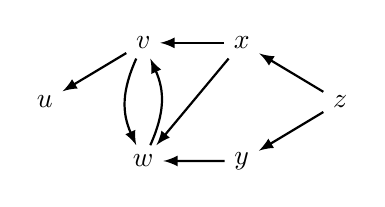
\begin{tikzpicture}[xscale=1.25, yscale=0.75]
      \node[vertex] (u) at (0, 0) {$u$};
      \node[vertex] (v) at (1, 1) {$v$};
      \node[vertex] (w) at (1, -1) {$w$};
      \node[vertex] (x) at (2, 1) {$x$};
      \node[vertex] (y) at (2, -1) {$y$};
      \node[vertex] (z) at (3, 0) {$z$};

      \draw[arrow] (v) to (u);
      \draw[arrow, bend right=15] (v) to (w);
      \draw[arrow, bend right=15] (w) to (v);
      \draw[arrow] (x) to (v);
      \draw[arrow] (x) to (w);
      \draw[arrow] (y) to (w);
      \draw[arrow] (z) to (x);
      \draw[arrow] (z) to (y);
    \end{tikzpicture}
    \caption{A conflict graph}\figlabel{ExamplePreCondensation}
  \end{subfigure}

  \begin{subfigure}[b]{0.3\textwidth}
    \centering
    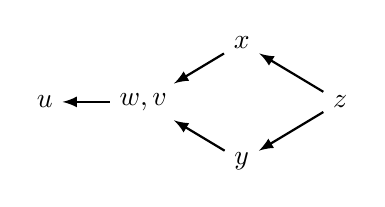
\begin{tikzpicture}[xscale=1.25, yscale=0.75]
      \node[vertex] (u) at (0, 0) {$u$};
      \node[vertex] (vw) at (1, 0) {$w,v$};
      \node[vertex] (x) at (2, 1) {$x$};
      \node[vertex] (y) at (2, -1) {$y$};
      \node[vertex] (z) at (3, 0) {$z$};

      \draw[arrow] (vw) to (u);
      \draw[arrow] (x) to (vw);
      \draw[arrow] (y) to (vw);
      \draw[arrow] (z) to (x);
      \draw[arrow] (z) to (y);
    \end{tikzpicture}
    \caption{The condensed conflict graph}\figlabel{ExampleCondensation}
  \end{subfigure}

  \caption{A conflict graph.}\figlabel{ExampleConflictGraph}
\end{floatingfigure}
}

The BPaxos protocols reach consensus on a conflict graph by first reaching
consensus on a partial instance graph. When a client sends a command to a
BPaxos protocol, the command is eventually assigned a unique instance $I$ and a
set of instances, $\deps{I}$, called the \defword{dependencies} of $I$. The
BPaxos protocols then reach consensus on instance $I$, choosing a command $x$
and set of dependencies $\deps{I}$ for instance $I$ once and for all. Every
replica $r_i$ maintains a partial instance graph $G_i$, and when the replica
learns that an instance $I$ has been chosen with command $x$ and dependencies
$\deps{x}$, it adds vertex $I$ to $G_i$ labelled with $x$ and with outbound
edges to every instance in $\deps{I}$ (adding previously unknown instances as
necessary).

Replica $r_i$ also maintains the eligible suffix $S_i$ of $G_i$ as well as the
\defword{condensation} $C_i$ of $S_i$. The condensation of $S_i$ is the graph
obtained by first removing spurious edges between non-conflicting vertices in
$S_i$ and then by contracting every strongly connected component. Every
strongly connected component consisting of commands $x_1, \ldots, x_n$ is
replaced with a single vertex labelled with a command string $x_{i_1} x_{i_2}
\cdots x_{i_n}$ that is obtained from a predetermined ordering of the commands
$x_1, \ldots, x_n$. An example condensation is shown in \figref{Condensation}.
%
Every $C_i$ is a conflict graph with respect to $\Cmd^+$ and $\conflict^+$
where $\Cmd^+$ is the set of non-empty command strings and where $(x_1 x_2
\cdots x_n, y_1 y_2 \cdots y_m) \in \conflict^+$ if there exists an $x_i$ and
$y_j$ that conflict in $\conflict$. To achieve consensus on these conflict
graphs, it suffices to maintain the following two invariants:

\begin{invariant}\invlabel{ConsensusInvariant}
  Once a command $x$ and set of dependencies $\deps{I}$ are chosen in instance
  $I$, no other command and set of dependencies can be chosen.
\end{invariant}
\begin{invariant}\invlabel{ConflictInvariant}
  If $(x, \deps{I_1})$ are chosen in instance $I_1$ and $(y, \deps{I_2})$ are
  chosen in instance $I_2$, and if $x$ and $y$ conflict, then either $I_1 \in
  \deps{I_2}$ or $I_2 \in \deps{I_1}$ or both.
\end{invariant}

\invref{ConsensusInvariant} states that consensus is reached for every
instance. This allows replicas to reach consensus on a partial instance graph.
\invref{ConflictInvariant} states that there must exist an edge between
vertices labelled with conflicting commands in the instance graph. This
suffices to ensure that every replica's instance graph really is an instance
graph.

The BPaxos protocols guarantee nontriviality in a straightforward way. They
guarantee stability because a replica's partial instance graph (and hence its
condensation) only grows over time. They guarantee stability because the
condensations of any two replicas' partial instance graphs are always a prefix
of the condensation of the union of their two partial instance graphs. Assuming
the possibility of only a single node failure, guaranteeing liveness is
impossible~\cite{fischer1982impossibility}. The BPaxos protocols do provide
liveness with certain assumptions about the niceness of the network, but we do
not focus on liveness in this paper.

Every BPaxos protocol follows this structure of reaching consensus on a partial
instance graph one vertex at a time and locally computing condensations of
eligible suffixes. The protocols differ only in how they compute dependencies
and how they reach consensus on a given instance. Thus, to prove the
correctness of a BPaxos protocol, it suffices to prove that the protocol
maintains \invref{ConsensusInvariant} and \invref{ConflictInvariant}.
